\documentclass[stu, 12pt]{apa7}
\usepackage{tabularray}
\usepackage{float}
\usepackage{graphicx}
\usepackage{codehigh}
\usepackage[normalem]{ulem}
\UseTblrLibrary{booktabs}
\UseTblrLibrary{siunitx}
\newcommand{\tinytableTabularrayUnderline}[1]{\underline{#1}}
\newcommand{\tinytableTabularrayStrikeout}[1]{\sout{#1}}
\NewTableCommand{\tinytableDefineColor}[3]{\definecolor{#1}{#2}{#3}}

\title{The Economic Outcomes of Corruption}
\author{Júlia Quintaneiro Pimenta}
\affiliation{\mbox{Master in Social Sciences, Universidad Carlos III de Madrid}}
\course{C4.325.19303-1: Applied Quantitative Methods for the Social Sciences I}
\professor{Francisco Villamil Fernandez}
\duedate{30 April 2026}

\begin{document}

\maketitle

An OLS regression was run to examine the relationship between the level of corruption and 
economic output, measured in GDP per capita. Table 1 and Figure 1 below show the key results.

\begin{table}
\caption{Regression Results}
\centering
\begin{talltblr}[         %% tabularray outer open
entry=none,label=none,
note{}={+ p \num{< 0.1}, * p \num{< 0.05}, ** p \num{< 0.01}, *** p \num{< 0.001}},
]                     %% tabularray outer close
{                     %% tabularray inner open
colspec={Q[]Q[]Q[]},
hline{2}={1-3}{solid, black, 0.05em},
hline{6}={1-3}{solid, black, 0.05em},
hline{1}={1-3}{solid, black, 0.08em},
hline{15}={1-3}{solid, black, 0.08em},
column{2-3}={}{halign=c},
column{1}={}{halign=l},
}                     %% tabularray inner close
& GDP & log GDP \\
(Intercept) & \num{-6819.280}*** & \num{6.798}*** \\
& (\num{1097.390}) & (\num{0.125}) \\
ti\_cpi & \num{3893.006}*** & \num{0.421}*** \\
& (\num{313.203}) & (\num{0.024}) \\
Num.Obs. & \num{170} & \num{170} \\
R2 & \num{0.673} & \num{0.603} \\
R2 Adj. & \num{0.671} & \num{0.600} \\
AIC & \num{3428.3} & \num{3267.1} \\
BIC & \num{3437.7} & \num{3276.5} \\
Log.Lik. & \num{-1711.134} & \num{-184.912} \\
F & \num{154.496} & \num{320.113} \\
RMSE & \num{5690.52} & \num{0.72} \\
Std.Errors & HC3 & HC3 \\
\end{talltblr}
\end{table}


\begin{figure}[H]
    \centering
    \caption{Scatter Plot}
    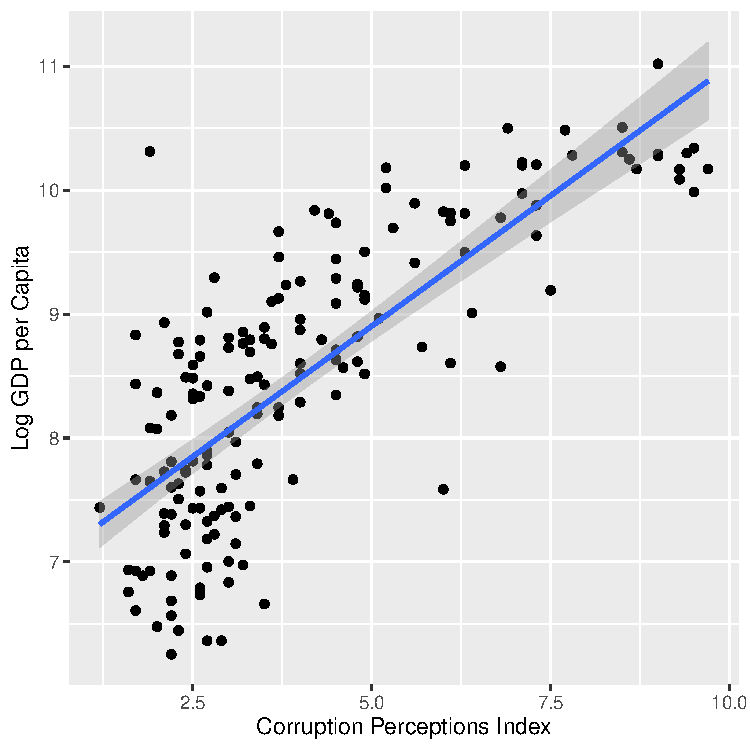
\includegraphics{corruption_log.pdf}
\end{figure}

\end{document}